\documentclass[pdftex,12pt,a4paper]{article}
\usepackage[english]{babel}
\usepackage{graphicx}
\usepackage[margin=2.5cm]{geometry}
\usepackage{fancyhdr}
%\usepackage[T1]{fontenc}
\usepackage{setspace}
\usepackage{multirow}
\usepackage{multicol}
\usepackage{mathtools}
\usepackage{amssymb}
\usepackage{caption}
\usepackage{url}
\usepackage{tikz}
\usetikzlibrary{arrows,decorations.markings,shapes}
\usepackage{array}
\usepackage{booktabs}
\usepackage{multirow}
\usepackage{pgfplots}
\usepackage{float}
\usepackage[font={footnotesize}]{caption}
\usepackage{graphicx}
\usepackage{todonotes}
\usepackage[font={footnotesize}]{subcaption}
\usepackage{listings}
%\usepackage[framed,numbered,autolinebreaks]{mcode}
\usepackage{graphicx,xcolor,textpos}
\usepackage{helvet}
\usepackage{color} %red, green, blue, yellow, cyan, magenta, black, white
\definecolor{mygreen}{RGB}{28,172,0} % color values Red, Green, Blue
\definecolor{mylilas}{RGB}{170,55,241}

%tikz stuff
\newlength\figureheight
\newlength\figurewidth

\pagestyle{fancy}
\lhead{Reports: Artificial Neural Networks}
\rhead{2015-2016}



\begin{document}


\section{PROJECT 1: Regression of function data}\label{sec:regression}
The data stems from a non linear function. Hence, a non-linear transfer function is required. Bearing in mind the results of Lehno \textit{et al.}, I find that the \texttt{tansig} (non-polynomial) function for the hidden layers must allow a function approximation if the number of neurons is sufficient. For the output layer, I use a \textit{purelin} transfer function, which does not restrict the output values to a particular range of values. In most cases, a single layer neural network is sufficient to reproduce a function (in theory, it is sufficient for \textit{all} functions if the number of neurons is large enough). Hence, we start with a single layer. Since the typical Euclidian distance between data points is small compared to the typical spacial structure dimension in addition to the fact that the data has not been jittered, the number of neurons can be taken to be relatively high without overfitting. To get an estimate of the number of neurons, we refer to Fig.~\ref{fig:performance_val}. We note that by considering the validation set performance, the optimal number of neurons is between $25 - 40$. Note that at this stage, we may not consider the test set performance. We opt for $35$ neurons. Note that to generate Fig.~\ref{fig:performance_val}, we did not use the validation set in a stopping criterion. This is because we want to \textit{detect} overfitting, rather than \textit{avoiding} it. The latter is the subject of the next paragraph.

First, we discuss the purpose of the data sets. Training is done on the training set, meaning that the network-parameters are varied such that it reproduces the training set with an overall error which is as small as possible. When the network starts to overfit the training data, the error on the validation set typically begins to rise. This indicates that the network is adjusted in such a way that it minimizes the error with respect to the training set, while having bad generalization properties in the regions where no training data is available. Therefore, when the validation error increases for a specified number of iterations (\texttt{net.trainParam.max\_fail} = 20), the training is stopped, and the weights and biases at the minimum of the validation error are returned. The test set only serves as a final check and cannot be used in the training and validation process.

\begin{figure}[tbh]
\centering
\begin{minipage}{0.4\textwidth}
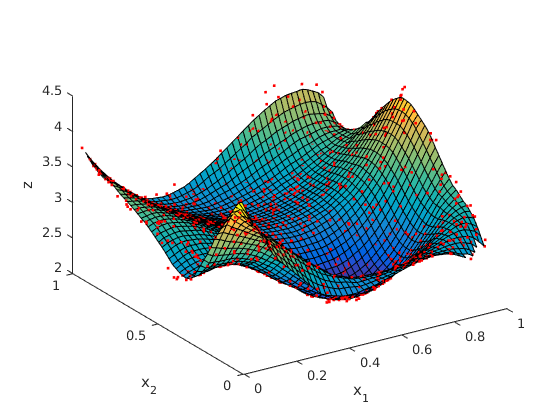
\includegraphics[height=5cm]{figs/train_surface.png}
\end{minipage}\quad
\begin{minipage}{0.4\textwidth}
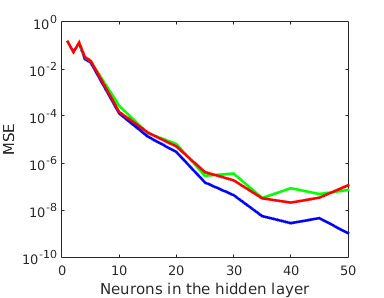
\includegraphics[height=5cm]{figs/performance_val.png}
\end{minipage}
\caption{Left: surface and data points in the training set. Right: Performance on the training, validation and test set as a function of the number of neurons in the hidden layer. \label{fig:performance_val}}
\end{figure}

\begin{figure}[tbh]
\centering
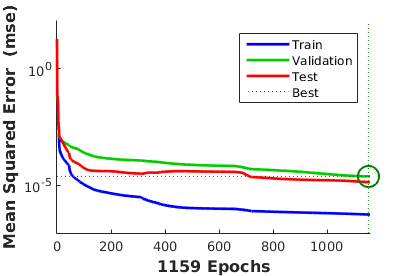
\includegraphics[height=5cm]{figs/MSE_final.png}
\caption{Performance on the training, validation and test set as a function of the number of epochs in the training process. \label{fig:MSE_final}}
\end{figure}

\begin{figure}[tbh]
\centering
\begin{minipage}{0.5\textwidth}
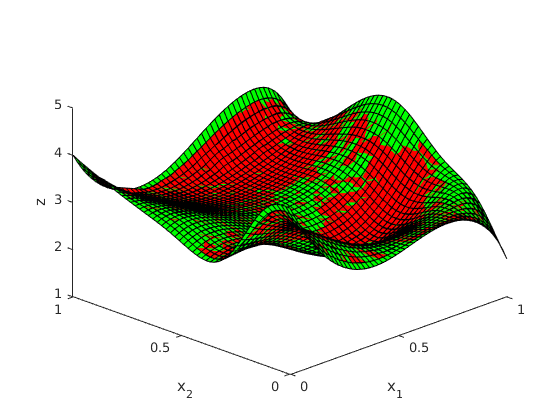
\includegraphics[height=5cm]{figs/NN_and_testsurf.png}
\end{minipage}%
\begin{minipage}{0.5\textwidth}
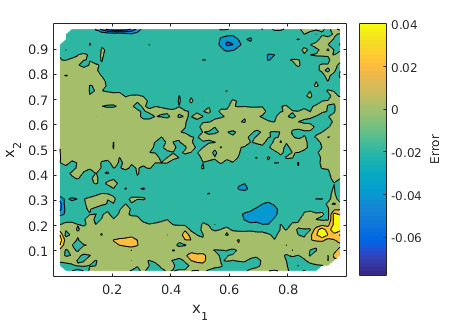
\includegraphics[height=5cm]{figs/NN_test_error.png}
\end{minipage}%
\caption{Left: Neural network (green) and test data (red) surface. The surfaces are almost indistinguishable. Right: Contour plot of the test set error. \label{fig:NN_and_testsurf}}
\end{figure}

The MSE on the test set of the resulting NN is $5.5 \times 10^{-5}$. We observe the pattern that the network has slightly higher values when the test set interpolation is large, and smaller values when the interpolations function is small. Hence, more extremal values are obtained.

To improve the results, we can use all of the provided data, instead of a subset of $3000$. Also, the data division does not need to be equal for all sets. As a rule of thumb, one generally assumes 70:15:15 (or 60:20:20) for the train:validation:test set ratios. This changes the MSE test error to $4.1\times10^{-8}$.

\section{PROJECT 2: Classification of wine data}\label{sec:classification}
Since it is not given whether or not the wine data is linearly separable, we use a non-linear model. We now use a \texttt{tansig} transfer function in the output layer, since this restricts the output to the domain $[-1,1]$ and the target output is in the format of $\pm 1$. We rescale the attributes to standardized values in order to make it independent of the scale of the data attributes. $15$ neurons in the hidden layer is optimal to classify the validation data. Using this architecture, a CCR of $0.60$  and $0.72$ is obtained for the validation and test set respectively. This might indicate that the two wine classes have a significant overlap in their attribute space.


\begin{figure}
\centering
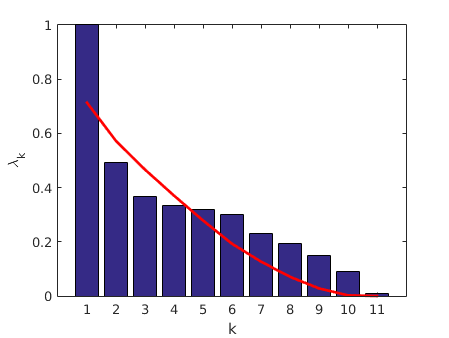
\includegraphics[width=6cm]{figs/eigenvalues.png}
\caption{Eigenvalues of the $11\times11$ covariance matrix. The red line indicates the cumulative sum of remaining (k+1):end eigenvalues, which is proportional to the reconstruction error. \label{fig:eigenvalues}}
\end{figure}

Next, the data is projected onto its lower dimensional principle component basis and reconstructed afterwards. The eigenvalue spectrum of the covariance matrix is depicted in Fig.~\ref{fig:eigenvalues}. Prior to computing the covariance matrix, we again rescale the data such that all attributes have zero mean and unit standard deviation. The eigenvalue spectrum does not show a clear dominant principle component. Hence, there is no clear indication that the data lives on a low-dimensional subspace. We take a reconstruction error of $10\%$, which corresponds with an $8$ dimensional basis. $11$ hidden neurons minimize the CCR of the validation set, which is less than before, as expected. Using this approach, a validation and test set CCR of $0.75$ and $0.72$ is obtained. Hence, there is a significant CCR increase for the validation set, while test set CCR is almost constant.

Hence, by projecting the data onto a lower dimensional space, a significant classification improvement of approximately $14 \%$ of the validation set is realized. However, the result is not true in general, since such a large increase is not found for the test set. This is related to the fact that the principle component basis is that of the training set, and is not updated if new data is included.

We remark that the possibility of overfitting is very real in this classification assignment. 

\newpage
\section{PROJECT 3: Character recognition}
\subsection{Hopfield network}
\begin{figure}[htb]
\centering
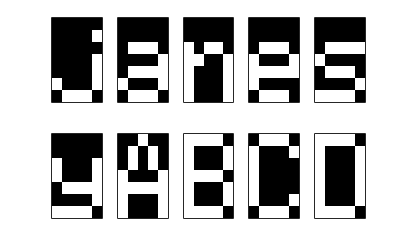
\includegraphics[width=10cm]{figs/letters.png}
\caption{First 10 of the 32 letters that are used in the character recognition exercise.\label{fig:letters}}
\end{figure}
In this section we train a Hopfield network to reconstruct the states in Fig.~\ref{fig:letters} from a distorted version of these characters. Hopfield networks are generated by providing it the undistorted images. 

\begin{figure}[htb]
\centering
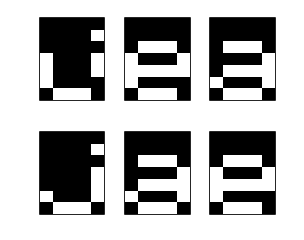
\includegraphics[width=10cm]{figs/wrong_states.png}
\caption{Incorrectly reconstructed characters (top row) with corresponding input (bottom row).\label{fig:wrong_states}}
\end{figure}

Figure~\ref{fig:wrong_states} illustrates a number of incorrectly reconstructed states with corresponding undistorted input. The `e' and `a' characters are often interchanged in the reconstruction. This is related to the fact that these characters have many pixels with the same value, and hence a similar shape. This means that the ridge in the energy function between these two attractor states is lower than the 3-pixel distortion. 
The incorrectly returned `j' character shows a spurious state which is a linear combination of multiple characters.
These cases are obtained when allowing for a sufficiently large number of time steps ($1000$). This allows one to observe the spurious states that are inherent to the system, rather than states that have not yet converged.

\begin{figure}[htb]
\centering
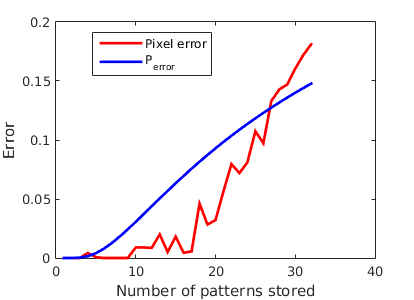
\includegraphics[width=8cm]{figs/Error_ifo_P.png}
\caption{Total pixel error (red),normalized over the number of states generated and total pixels in an image (35), and the theoretical prediction curve based on the Hebb rule (blue).\label{fig:error_ifo_P}}
\end{figure}

We now determine how number of patterns that are stored influence the number of erroneously restored characters. For each case of $P$ stored patterns, we create a Hopfield network and generate a sufficient number of 3-pixel distorted images. These are then reconstructed, after which we calculate the number of pixels that do not correspond to the original image. The results are shown in Fig.~\ref{fig:error_ifo_P}. On can observe a steep rise in the reconstructed pixel error after $P=17$. Hence, $17$ stored patterns is the critical loading capacity of the network. Naturally, when the number of distorted pixels is increased, this number is expected to go down. For $P$ larger than the critical loading capacity, the large number of spurious states and the small basins of attraction of attractor state do not allow for a reliable character restoration.

One can theoretically predict the dependence of the reconstruction error as a function of the number of patterns stored, using Hebbs' rule for uncorrelated patters. The prediction curve is also shown in Fig.~\ref{fig:error_ifo_P}. If we assume a large $P$ and large $N$, we obtain an estimated $P_{\textrm{error}}$
\begin{equation}
P_{\textrm{error}} = \frac{1}{\sqrt{2 \pi} \sigma} \int_{1}^{+\infty} e^{\frac{-x^2}{2 \sigma^2}} dx \,,
\end{equation}
where $\sigma=\sqrt{P/N}$. Hence, a first approximation is that $P$ and $N$ are large, which is not actually the case here. However, both the prediction and simulation show the same (expected) behaviour: first a flat $P$ dependence, followed by a steep rise. One can estimate the storage capacity from
\begin{equation}
P_{\max} = N/(4 \log N) =2.46 \,.
\end{equation}
Hence, for 2 or less stored patterns, the Hopfield should be able to perfectly reconstruct the distorted images.

One way to resolve the issue of incorrectly reconstructed images, is to increase the number of pixels in each  image. In the case at hand, each image is determined by $35$ pixels. Hence, it was expected that the critical loading capacity would be relatively low. By increasing the number of pixels in an image, each character has more attributes by which it is characterized. This is the obvious alternative to the current Hopfield network. In the next subsection we discuss another alternative.

\subsection{Alternative solution to character recognition}
The Hopfield network for character recognition is ``only implemented in MATLAB for historical reasons''. Nowadays, many more, and better ANNs are available on the market. Not only can one choose the architecture of the network, but also the error determination can be chosen to optimize the problem. Another choice is which input is used to train the network. It has been shown that (as expected), a network performs better in character restoration if it is trained with distorted input images. This is clearly illustrated in an example by Matlab \footnote{\url{http://nl.mathworks.com/help/nnet/examples/character-recognition.html}}.

The opted network architecture is as follows: we generate a feedforward neural network with one hidden layer of $25$ neurons and an output layer of dimension equal to the number of patterns $P$ that are to be stored. In the hidden layer, we use a \texttt{tansig} transfer function, while in the output layer, we use the \texttt{softmax} function. The final output is such that we put all output components to 0, except for the one with the maximum value, which is 1. Hence, we use one-hot encoding of the stored characters. This means that every character out of the $P$ stored characters is determined by a $P$-dimensional vector of zeros, except for a one in a unique place. Hence, also the actual characters must be stored such that one can return a character instead of this vector.  Note that the input still takes the $35$ pixels as in the original Hopfield network.

One-hot encoding is feasible if the number of patterns stored is not too large, since the size of the output layer is equal to the size of the alphabet to be stored.

In the previous subsection we showed that the ``e'' and ``a'' are difficult for the Hopfield network to restore correctly, since these characters have very similar features. Hence, if one would create a network that uses an $N=35$ dimensional output, similar problems would be faced, since these characters are only separated by a small distance in output space. In one hot-encoding, the distance between two patterns in output space is $\sqrt{2}$, independent of whether they have similar patterns.

We train our network with $100$ distorted images of each letter to be stored. We vary the number of patterns and determine the number of incorrectly restored patterns as a function of the number of patterns stored. We use a constant $25$ hidden neurons for practical reasons. The results are shown in Fig.~\ref{fig:alternative_error}. A steady rise is observed as expected.
\begin{figure}
\centering
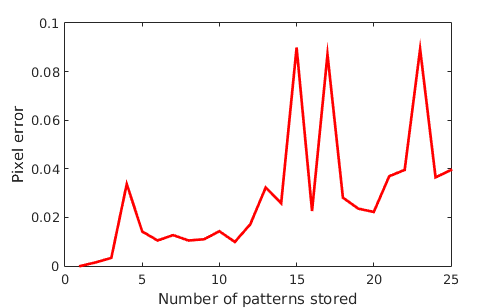
\includegraphics[width=10cm]{figs/alternative_error.png}
\caption{Percentage of false reconstructed images (not pixels as before) as a function of the number of patters stored.\label{fig:alternative_error}}
\end{figure}

Naturally, the networks' performance can easily be improved by increasing the number of neurons and/or hidden layers. In addition, approximately $6500$ possible 3-pixel distortions of each letter. Hence, in theory all possibilities can be generated to form the training batch. However, substantial computing resources are required if batch-training is required. We will not go into further detail, since these calculations are hard to perform on a simple laptop.


%%%%%%%%%%%%%%%%%%%%%%%%%%%%%%%%%%%%%%%%%%%%%%%%%%%%%%%%
\newpage
\appendix

%\lstset{style=Matlab-editor}
%
\lstset{language=Matlab,%
basicstyle=\small, %or \small or \footnotesize etc.
    %basicstyle=\color{red},
    breaklines=true,%
    morekeywords={matlab2tikz},
    keywordstyle=\color{blue},%
    morekeywords=[2]{1}, keywordstyle=[2]{\color{black}},
    identifierstyle=\color{black},%
    stringstyle=\color{mylilas},
    commentstyle=\color{mygreen},%
    showstringspaces=false,%without this there will be a symbol in the places where there is a space
    numbers=left,%
    numberstyle={\tiny \color{black}},% size of the numbers
    numbersep=9pt, % this defines how far the numbers are from the text
    emph=[1]{for,end,break},emphstyle=[1]\color{black}, %some words to emphasise
    %emph=[2]{word1,word2}, emphstyle=[2]{style},    
}

\section{Matlab code that implements the solutions}
\subsection{Regression (see Section \ref{sec:regression})}
\subsubsection{Main code}
\lstinputlisting{../regression/regression_project.m}
\subsection{Classification (see Section \ref{sec:classification})}
\subsubsection{Main code}
\lstinputlisting{../classification/classification.m}
\subsubsection{PCA related}
\lstinputlisting{../classification/doPCA.m}
\subsection{Classification (see Section \ref{sec:classification})}
\subsubsection{Main code}
\lstinputlisting{../hopfield/hopfield.m}
\subsubsection{Image distortion}
\lstinputlisting{../hopfield/DistortImage.m}
\subsubsection{Name generation}
\lstinputlisting{../hopfield/GenerateName.m}

\subsubsection{Alternative to Hopfield}
\lstinputlisting{../hopfield/alternative.m}


\end{document}